\documentclass[10pt, abstracton, twocolumn]{scrartcl}

\usepackage{simpleConference}
\usepackage{customTikz}
\usepackage{times}
\usepackage{graphicx}
\usepackage{tabularx}
\usepackage{amssymb}
\usepackage{hyperref}
\usepackage{url}
\usepackage{tikz}
\usepackage{amsmath}
\usepackage{gensymb}
\usepackage{varioref}
\usepackage[all]{hypcap}
\usepackage{subcaption}
\usepackage[toc,page]{appendix}
\usepackage[boxed]{algorithm2e}

\hypersetup{
  colorlinks=true,
  linkcolor=black,
  urlcolor=black,
  citecolor=black
}

\def\labelitemi{--}

\usetikzlibrary{calc}

\setcounter{secnumdepth}{3}
\setcounter{tocdepth}{2}

\SetAlCapSkip{0.15in}

\DeclareMathOperator{\dist}{d}
\DeclareMathOperator{\proj}{\phi}

\newcommand{\fref}[1]{\hyperref[#1]{figure \vref{#1}}}
\newcommand{\sref}[1]{section \vref{#1}: \nameref{#1}}
\newcommand{\aref}[1]{\hyperref[#1]{algorithm \vref{#1}}}
\newcommand{\link}[2]{\textsc{\href{#1}{#2}}}

\renewcommand{\arraystretch}{1.5}

\begin{document}

\thispagestyle{empty} % remove page number on this page

\onecolumn

\title{CONVOI Project Report \\
\vspace{.5em}
\normalsize{Camera-Operated Navigation and Vehicle-Object Interaction} }

\author{\textit{primary research and development} \\ 
Koen Dercksen \hspace{2em} Marein K\"onings \\
\\
\textit{team members} \\
Caspar Safarlou \hspace{2em} Chris Kamphuis \hspace{2em} Erik Verboom \\
\\
January 2014 \\
\\
for the course of Robotica II \\
taught by Perry Groot and Ida Sprinkhuizen-Kuyper \\
assisted by Bas Bootsma \\
\\
as part of Artificial Intelligence \\
at Radboud University, Nijmegen
}

\onecolumn

\maketitle

\thispagestyle{empty} % remove page number on this page

\begin{center}
\begin{minipage}{35em}

\begin{abstract}
With this report, we aim to explore the process of creating our image-recognition and planning software. We try to explain in detail the methods by which our program works and our reasons for choosing these particular methods. We examine both the physical and the software components that make up the system. Ideas and techniques that didn't make it into the final product are mentioned as well. Finally, we reflect on the development process.
\end{abstract}

\end{minipage}
\end{center}

\clearpage

\thispagestyle{empty} % remove page number on this page

\tableofcontents

\clearpage

\twocolumn

\section{Project Outline}

\subsection{The Assignment}
For the course of Robotica 2, we were presented with a very open-ended assignment, practically the only requirement being to design and implement some kind of task that was to be executed by multiple communicating robots. Unfortunately we failed to meet this core requirement due to circumstances described in \sref{sec:multiagent} and \sref{sec:team}.

Despite this one major shortcoming, we feel we have created a very interesting task and project, and that we have learned a lot developing it. We are excited to present to you in complete detail our algorithms and processes.

The assignment posed several secondary requirements, including wireless communication with a robot and the use of a version control system, which we did meet. Our primary areas of research and learning were computer vision and data management.

\subsection{Task and Execution}
We brainstormed about the task we wanted to execute for a long time. We knew that we wanted to do something that involved actual interdependence between the robots, not just a one-way interaction or no meaningful interaction at all. We also wanted to avoid having to work with the NXT sensors, after bad experiences from last year, and some people in our team were interested in exploring computer vision possibilities. Finally, we wanted to be able to distil our project to a very simple version to construct first, with the possibility of more complex additions later.

As it turned out, we were unable to construct even the distilled version of the project successfully. As such we will here be describing the task that the single robot was able to execute at the end of the project.

\begin{figure}[h]
        \centering
        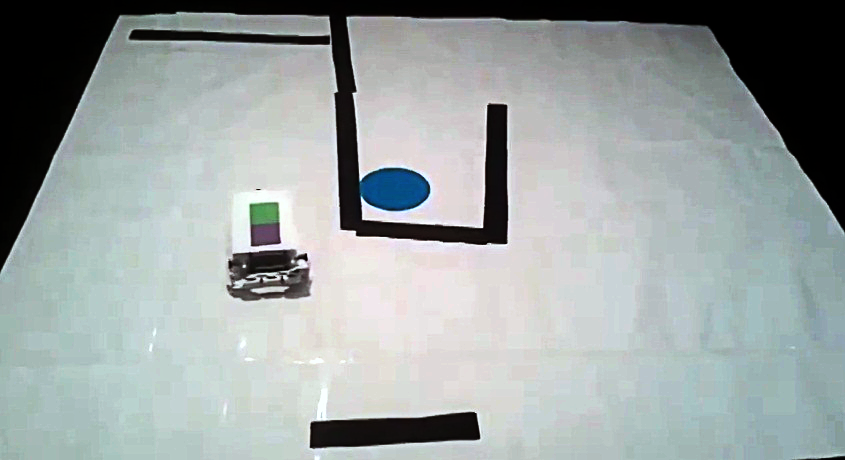
\includegraphics[width=\columnwidth]{pictures/photo1convoi.png}
        \caption{\small CONVOI in action}
        \label{fig:photo1convoi}
\end{figure}

\subsubsection{Primary goals}
A classic vehicle-like robot moves around on a large flat surface. A goal is located on this surface as well. The robot's task is to reach the goal. Also present on the surface are thick black strips of paper that represent the walls of a maze that the robot must navigate in order to reach the goal. Obviously, the robot is not allowed to pass over the black lines.

While the above describes the primary goal for our robot, a high-level goal for ourselves was to create our software in such a way that it would be able to handle changes in the environment. That is to say, we wanted any regular user to be able to change the maze by moving the and the locations of walls and the goal on the fly, without this forming a problem for the robot.

\subsubsection{Means}
In order to reach our goals, we must obtain some knowledge about the world. We have one single source of information about the world: a camera hanging above the playing field. Armed with only this, we must find a path for the robot to travel, using a host of interesting techniques from fields such as computer vision.

In order to facilitate object recognition, we use primary and secondary colours only. The type of a relevant object in the world can be recognized by the colour of that object.

We require a direct connection to the robot at all times, allowing us to send it motor orders.

\section{Third-Party Software}
Like any project of this scope, we relied heavily on work done by others to achieve our goals. All external software that we used and parts of our program that we did not write ourselves are listed below. These fall into two main categories; software that we used to develop our code, and the libraries and algorithms that we incorporated into our code.

\subsection{Development Tools}
We feel that, in any programming project, especially when working in teams, there are three choices to make when it comes to development tools. The first and most obvious is the choice of programming language. While this may in many cases be constrained by the nature of the project, we were free to choose. When a language is chosen, an appropriate integrated development environment (IDE) should be selected in order to facilitate working with the language. Finally, in order to safely store one's work and have the ability to revert changes, a version control system (VCS) should be chosen. This is relevant especially when working in a team, since a good VCS also simplifies the process of integrating work from different people into the codebase.

Below, we explain the choices that we have made in these three categories.

\subsubsection{C\#}
C\# is a primarily object-oriented programming language developed by Microsoft. C\# is like Java in many ways, which allowed us to start using it without needing much time to adapt. We chose to work with C\# during this project mainly because of our initial plans to use Microsoft Robotics Studio.

\subsubsection{Visual Studio}
Microsoft Visual Studio is by far the most popular C\# IDE around. It offers various powerful tools such as a GUI editor, IntelliSense, performance analysis and a whole lot more. A good IDE is very important in software development in order to maintain sanity, so we went with Visual Studio.

\subsubsection{Git}
Version control is very important in team efforts. It allows all members of the team to work on the same code in a safe manner, and provides a way to roll back to earlier versions (to find out where a bug was introduced for example) if necessary. Version control systems in combination with an online repository host improve the mobility of the code; just get the latest version from wherever you are and start working.

We chose Git because it is a very fast and lean but powerful version control system that various people in the team had already used before.

\subsection{Libraries and Algorithms}
As part of our project, we used several third-party libraries in our code to solve certain problems. We also made use of (mathematical) algorithms from online sources. All of these are listed below, including our reasoning for using the software rather than writing our own. In most of these cases, a primary factor was a need not to 'reinvent the wheel'. Of course we only applied this reasoning to problems that we didn't find interesting, as we did write our own code in other areas of the project. We would like to note that we have solid ideas on how we would ourselves solve most of the problems below.

\subsubsection{Logitech Camera Software}
The webcam we used, the Logitech QuickCam Pro 9000, comes with specialized software that includes the ability to set such properties as zoom, focus, contrast and colour intensity. We use this software to pre-process the webcam input, removing noise and turning it into something that is more easily analysed by our software. The effect of pre-processing can be seen in \fref{fig:preprocessing}.

\begin{figure}[h]
        \centering
        \begin{subfigure}[t]{0.45\columnwidth}
        \centering
        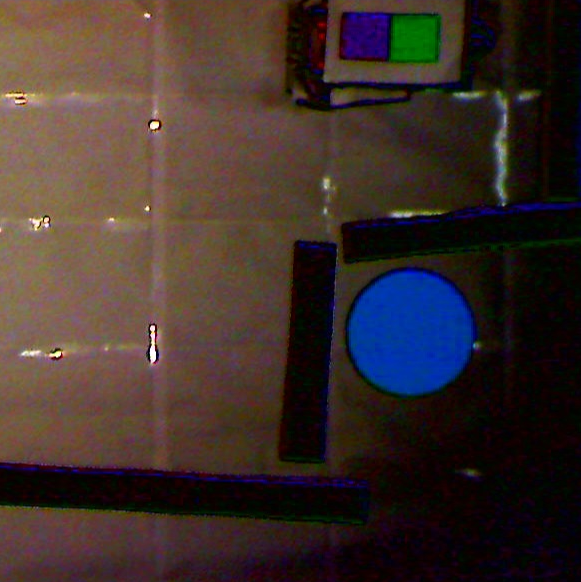
\includegraphics[width=\columnwidth]{pictures/preprocessing1.png}
        \end{subfigure}
        \begin{subfigure}[t]{0.45\columnwidth}
        \centering
        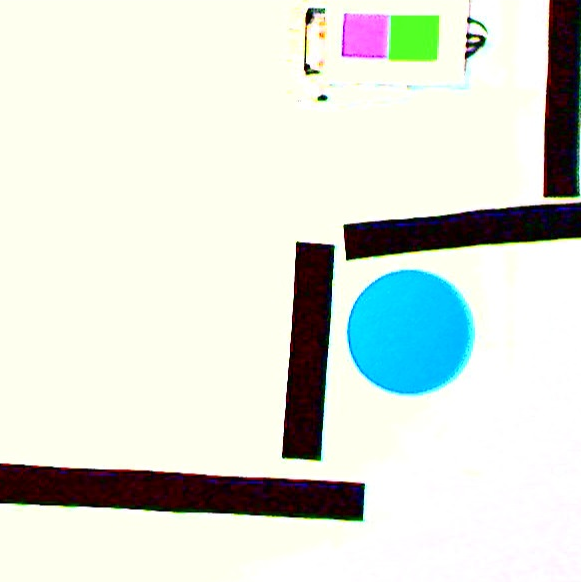
\includegraphics[width=\columnwidth]{pictures/preprocessing2.png}
        \end{subfigure}
        \caption{\small Webcam input before and after pre-processing.}
        \label{fig:preprocessing}
\end{figure}

We were initially unaware of the Logitech software, and considered writing our own code for pre-processing. We decided this was too much effort compared to the gain, especially since our analysis software was able to handle input without pre-processing. When we discovered the Logitech software and the ease with which it allowed us to preprocess the input, we decided to use it into our analysis pipeline to further prevent errors.

\subsubsection{EmguCV}
\link{http://www.emgu.com/wiki/index.php/Main_Page}{EmguCV} is a .NET wrapper of OpenCV, an image processing library developed by Intel. It offers a wide range of functionality from image and motion detection to machine learning algorithms. We only utilize a very small part of its functionality.

\paragraph{Camera Connection}
The wrapper contains methods for very easily communicating with a connected camera. Only a couple of lines of code are needed to establish a streaming input connection. We didn't anticipate EmguCV to contain this functionality, but we were very glad to discover this as it covered our needs completely.

We also set up a 'mock' input stream, which supplied predetermined images to the analysis pipeline. This mock input stream proved very useful for testing purposes, especially at times when we didn't have access to the robots or camera.

\paragraph{Contour Detection}
An important step in our analysis is the conversion of blobs to contours describing the shape of the blobs. Blobs are defined by a binary bitmap, defining one or multiple contiguous regions known as blobs. Contours are defined as polygons that (roughly) describe the shape of blobs. Important to note is that blob geometry is converted from a bitmap representation to an approximated vector representation. The result of the process can be seen in \fref{fig:contourDetection}.

\begin{figure}[h]
        \centering
        \begin{subfigure}[t]{0.45\columnwidth}
        \centering
        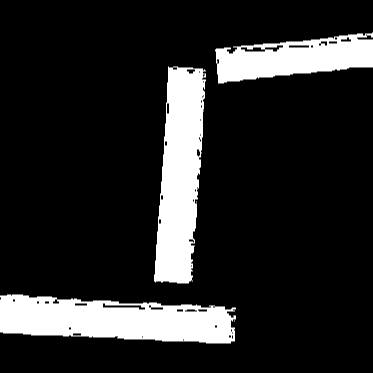
\includegraphics[width=\columnwidth]{pictures/contourDetection1.png}
        \end{subfigure}
        \begin{subfigure}[t]{0.45\columnwidth}
        \centering
        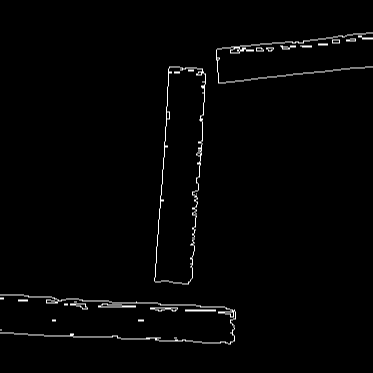
\includegraphics[width=\columnwidth]{pictures/contourDetection2.png}
        \end{subfigure}
        \caption{\small Blobs and corresponding contours.}
        \label{fig:contourDetection}
\end{figure}

EmguCV contains functionality to do exactly this, allowing some control over the algorithm used. We found the contour-finding algorithm known in EmguCV as LINK\_RUNS led to the best results in our situation. Unfortunately we have not found any documentation on the inner workings of the algorithm, and \link{https://github.com/Itseez/opencv/blob/bad927325fc9b73ad449fd46f8856a2cea448390/modules/imgproc/src/contours.cpp\#L129}{the source code} does not grant much insight.

\paragraph{Minimum Area Rectangle}
Many of the items we are detecting are rectangular, but may not appear exactly rectangular in the input (due to perspective and colour matching inaccuracies). As such, it is convenient to have a method of easily converting an arbitrary contour, which we have already established to represent a rectangular item, to a rectangular contour. EmguCV's 'minimum area rectangle' (MinAreaRect) functionality solves this problem for us.

Much like the common principle of a 'bounding box', the MinAreaRect is a rectangular box around a collection of points, such that the box contains all points, and the box could not be any smaller while still containing all points. Contrary to a regular bounding box, a MinAreaRect is not necessarily aligned to the Cartesian axes. This means that the MinAreaRect of a particular contour usually has a smaller area than the bounding box of that same contour, as the rotation of the rectangle allows for a more optimal fit. The principles of bounding boxes and minimum area rectangles are illustrated in \fref{fig:minAreaRect}.

\begin{figure}[h]
        \centering
        \begin{subfigure}[t]{0.30\columnwidth}
        \centering
        \begin{tikzpicture}[thick,scale=0.1, every node/.style={scale=1}]

\draw [line width=2,line cap=round,fill=yellow!15!white,rounded corners=.25ex] (1,0) -- (0,5) -- (2,10) -- (7,11) -- (8,15) -- (12,13) -- (9,6) -- (4,5) -- cycle;

\end{tikzpicture}
        \subcaption{\small A contour.}
        \end{subfigure}
        \begin{subfigure}[t]{0.30\columnwidth}
        \centering
        \begin{tikzpicture}[thick,scale=0.1, every node/.style={scale=1}]

\draw [lightgray,line width=2,line cap=round,fill=yellow!15!white,rounded corners=.25ex] (1,0) -- (0,5) -- (2,10) -- (7,11) -- (8,15) -- (12,13) -- (9,6) -- (4,5) -- cycle;

\draw [black,line width=2,line cap=round,dashed,rounded corners=.25ex] (0,0) -- (0,15) -- (12,15) -- (12,0) -- cycle;

\end{tikzpicture}
        \subcaption{\small The bounding box of the contour, with an area of 10 units$^2$.}
        \end{subfigure}
        \begin{subfigure}[t]{0.30\columnwidth}
        \centering
        \begin{tikzpicture}[thick,scale=0.1, every node/.style={scale=1}]

\draw [lightgray,line width=2,line cap=round,fill=yellow!15!white,rounded corners=.25ex] (1,0) -- (0,5) -- (2,10) -- (7,11) -- (8,15) -- (12,13) -- (9,6) -- (4,5) -- cycle;

\draw [black,line width=2,line cap=round,dashed,rounded corners=.25ex] (9.38,16.15) -- (-3.51,5.41) -- (1.33,-0.39) -- (14.21,10.34) -- cycle;

\end{tikzpicture}
        \subcaption{\small The minimum area rectangle of the contour, with an area of 7 units$^2$.}
        \end{subfigure}
        \caption{\small Illustration of bounding box and minimum area rectangle.}
        \label{fig:minAreaRect}
\end{figure}

In our implementation, with items that we know to be rectangles, the MinAreaRect is simply taken as the actual shape of the item. We were again unable to find information on the algorithm used.

\paragraph{Convex Hull}
The convex hull of a set of points is the smallest subset that defines a convex polygon, such that the polygon contains all of the original points. Practically, the original set of points may be seen as a polygon, and the convex hull is a modification of that polygon with all concavities removed, resulting in a convex polygon. An example of convex hull generation can be seen in \fref{fig:convexHull}.

\begin{figure}[h]
        \centering
        \begin{tikzpicture}[thick,scale=0.3, every node/.style={scale=1}]

\draw [lightgray,line width=8,line cap=round,fill=yellow!15!white,rounded corners=.25ex] (1,0) -- (0,5) -- (2,10) -- (7,11) -- (8,15) -- (12,13) -- (9,6) -- (4,5) -- cycle;

\draw [black,line width=2,line cap=round,dashed,rounded corners=.25ex] (1,0) -- (0,5) -- (2,10) -- (8,15) -- (12,13) -- (9,6) -- cycle;

\end{tikzpicture}
        \caption{\small Convex hull of the polygon seen in \fref{fig:minAreaRect}.}
        \label{fig:convexHull}
\end{figure}

We apply EmguCV's method for determining the convex hull of a polygon on contours, when we are looking for items that we know to have a convex shape. This accounts for some errors in colour matching, where part of an object was not detected as belonging to the object, resulting in a concave shape. This concave shape is made convex by converting to convex hull, removing the concavity that was missed in detection. Documentation on the algorithm is again lacking (\link{https://github.com/Itseez/opencv/blob/ef91d7e8830c36785f0b6fdbf2045da48413dd76/modules/imgproc/src/convhull.cpp\#L129}{source code}).

\paragraph{EmguCV Representation}
EmguCV uses its own data formats for almost all of its functionality. Since we are using this functionality in key areas of our pipeline, we came to use those data formats in many places ourselves. This includes the representation of polygons and images, and all associated representations such as points and colours.

However, there are two problems with this established setup, both to do with performance issues. These are listed in \sref{sec:emgucvFormats}, as there were plans for a better solution.

\subsubsection{Triangle.NET}
\link{http://triangle.codeplex.com/}{Triangle.NET} is a library that facilitates (Delauney) triangulation. Triangulation is the process of taking a polygon and dividing it up into triangles. This technique is a key part of our navigation mesh construction. Because of the key role of triangulation, and because we found it to be a difficult problem, and such a perfectly-suited library exists, we chose to use this software to perform all necessary triangulation operations. A display of polygon triangulation can be seen in \fref{fig:triangulation}.

\begin{figure}[h]
        \centering
        \begin{tikzpicture}[thick,scale=0.3, every node/.style={scale=1}]

\draw [lightgray,line width=8,line cap=round,fill=yellow!15!white,rounded corners=.25ex] (1,0) -- (0,5) -- (2,10) -- (7,11) -- (8,15) -- (12,13) -- (9,6) -- (4,5) -- cycle;

\draw [black,line width=2,line cap=round,dashed,rounded corners=.25ex] (1,0) -- (0,5) -- (2,10) -- (7,11) -- (8,15) -- (12,13) -- (9,6) -- (4,5) -- cycle;

\draw [black,line width=2,line cap=round,dashed,rounded corners=.25ex] (0,5) -- (4,5);

\draw [black,line width=2,line cap=round,dashed,rounded corners=.25ex] (2,10) -- (4,5);

\draw [black,line width=2,line cap=round,dashed,rounded corners=.25ex] (7,11) -- (4,5);

\draw [black,line width=2,line cap=round,dashed,rounded corners=.25ex] (7,11) -- (9,6);

\draw [black,line width=2,line cap=round,dashed,rounded corners=.25ex] (7,11) --  (12,13);

\end{tikzpicture}
        \caption{\small Triangulation of the polygon seen in \fref{fig:minAreaRect}.}
        \label{fig:triangulation}
\end{figure}

\subsubsection{AForge.NET}
\link{http://www.aforgenet.com}{AForge.NET} is a C\# framework containing implementations of various A.I. related algorithms and applications such as image processing, neural networks, machine learning and robotics. We used a very small part of this framework to communicate with the LEGO NXT Brick. AForge.NET handles the bluetooth connection with the brick and supplies convenient methods to issue motor commands.

\subsubsection{Native NXT Firmware}
LEGO NXT Bricks come with LEGO's own firmware. Since AForge.NET was built with this in mind, we did not have to flash the brick with a different type of firmware.

\subsubsection{Algorithms}
Next to libraries, our project incorporates many code snippets that we found on the internet. Most if not all of these are specific mathematical or geometric operations (e.g. the angle between two vectors or the centroid of a polygon). In our code, all of the instances where we copy-pasted a third-party snippet contain a reference to the source. In total there are 12 such references.

\section{Design and Implementation}
Our program is set up in a very linear way and divided up into clearly separated modules. First of all, a subscription is made to the camera such that, each time a new image is captured, a chain of functionality is initiated that is known as the analysis pipeline. The course of this pipeline is illustrated in \fref{fig:programOverview}. The pipeline analyses the image and culminates into a single location that the robot is meant to move towards as a first step in reaching the goal.

Meanwhile, a connection to the robot was established. At the end of the analysis pipeline, the resulting location is presented to the robot control system, which determines the precise motor commands to sent to the robot, in order to reach the location.

All of the steps in the analysis and control pipeline communicate with two further components: the interface and the Constants. The interface are a couple of windows where intermediate results of calculations are displayed for debugging purposes, and by which the user interact with the program (e.g. during colour calibration). The Constants is the collection of values that modify the behaviour of the program, such as the calibrated colours and the dimensions of the robot.

\begin{figure}[h]
        \begin{center}
        \begin{tikzpicture}[thick,scale=0.8, every node/.style={scale=0.8}]

\newcommand{\leftcol}{-3}
\newcommand{\rightcol}{3}

\draw [black,fill=yellow!15!white] plot [smooth, tension=.3] coordinates {(\leftcol+2,1) (\leftcol+2.5,0.5) (\rightcol-2.5,-3.675) (\rightcol-2,-4.175) (\rightcol-2,-5.325) (\rightcol-2.5,-5.825) (\leftcol+2.5,-10) (\leftcol+2,-10.5)};	

\draw [rounded corners=1ex,fill=yellow!15!white]
	(\leftcol-2,2) --
	(\leftcol+2,2) --
	(\leftcol+2,-11.5) --
	(\leftcol-2,-11.5) --
	cycle;

\ArrowNodeEnd{\leftcol}{9*-1.15}{Robot Control}
\ArrowNode{\leftcol}{8*-1.15}{Communication}
\ArrowNode{\leftcol}{7*-1.15}{Pathing}
\ArrowNode{\leftcol}{6*-1.15}{Navigation mesh}
\ArrowNode{\leftcol}{5*-1.15}{Object matching}
\ArrowNode{\leftcol}{4*-1.15}{Contour detection}
\ArrowNode{\leftcol}{3*-1.15}{Colour extraction}
\ArrowNode{\leftcol}{2*-1.15}{Colour calibration}
\ArrowNode{\leftcol}{1*-1.15}{Pre-processing}
\ArrowNodeStart{\leftcol}{0*-1.15}{Camera}
	
\node at (\leftcol,1.25) {\large\bf Analysis pipeline};

\draw [rounded corners=1ex,fill=yellow!15!white]
	(\rightcol-2,-3.175) --
	(\rightcol+2,-3.175) --
	(\rightcol+2,-6.325) --
	(\rightcol-2,-6.325) --
	cycle;
		
\draw [rounded corners=1ex, fill=white]
	(\rightcol-1.5,-3.675) --
	(\rightcol+1.5,-3.675) --
	(\rightcol+1.5,-4.675) --
	(\rightcol-1.5,-4.675) --
	cycle;
	
\node at (\rightcol,-4.175) {Interface};
			
\draw [rounded corners=1ex, fill=white]
	(\rightcol-1.5,-4.825) --
	(\rightcol+1.5,-4.825) --
	(\rightcol+1.5,-5.825) --
	(\rightcol-1.5,-5.825) --
	cycle;
		
\node at (\rightcol,-5.325) {Constants};

\end{tikzpicture}
        \end{center}
        \caption{\small Program design overview.}
        \label{fig:programOverview}
\end{figure}

In many steps of the analysis pipeline, the concept of 'object types' is important. These represent the different objects that can be detected by the program. Each of these types requires a unique colour. The object types relevant to the final project are listed below (there are more object types present in the code, due to plans for extensions. See \sref{sec:multiagent}).

\begin{itemize}
  \item Wall
  \item Goal
  \item Robot: A generic square that is placed on all robots
  \item TransportRobot: A square placed specifically on the transport robot (the only robot in use in the final design)
\end{itemize}

\subsection{Camera input}
We request the camera to provide us with images with a size of 1024 by 768 pixels. The higher the resolution, the lower the frame rate. We aimed for an analysis rate of three frames per second, and the chosen resolution enables the camera to provide images at three frames per second or higher. Each time the camera has captured an image, it activates the analysis pipeline, resulting (in most cases) in a new command being sent to the robot.

\subsection{Image Pre-processing}
The Logitech camera software enables us to apply a number of pre-processing modifications to the input image. The most important of these were the zoom, focus distance, exposure, gain, brightness, contrast, colour intensity and white balance of the image. Most of these needed to be manually re-calibrated whenever there was a change in the physical environment.

% picture of exposed settings: http://tdcat.com/wp-content/uploads/2013/03/makemostofskype_c920settings.png

\subsection{Colour Calibration}
Obviously, an important aspect of the analysis is knowing which colours signify which objects in the world. For the program to learn this, the user needs to calibrate the colour-object associations. The program then uses this information for all subsequent operations until the user performs a new calibration.

\subsubsection{Calibration Interface}
Calibration begins with choosing an object type to calibrate the colour of. The live pre-processed image is presented, and the user can click on it to indicate spots that should be seen as the colour of the chosen object type. In these spots, dots appear to indicate that the spot was clicked. These dots are of a fixed size which is of importance, as all pixels that are covered by the spot are seen as belonging to the chosen object type. A snapshot of the calibration process can be seen in \fref{fig:calibrationSpots}.

\begin{figure}[h]
        \centering
        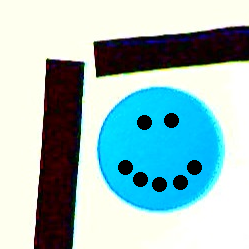
\includegraphics[width=\columnwidth]{pictures/calibrationSpots.png}
        \caption{\small Multiple selected spots for calibrating the goal colour.}
        \label{fig:calibrationSpots}
\end{figure}

Multiple spots can be clicked to cover a particular object as much as possible, or to cover multiple objects of the same type.

When the user has clicked all spots belonging to a certain object type (or as much as they deem sufficient to calibrate the colour), they can click a button to indicate they are finished. All pixels that were covered by dots are now used as calibration data in the calibration calculation (see below), and the results of this calculation are associated with the chosen object type. The user can now choose the next object type to calibrate.

Once all object types have been calibrated, the user can choose to save the set of calibrated values to a file. This file can then be loaded at a later time, sparing the user the effort of calibrating the values over again. Of course this is only a valid shortcut if the user is running the program under the same physical conditions as when saving the file. Otherwise, the colours of objects, as perceived by the webcam, may have changed.

\subsubsection{Calibration Calculation}

The calibration calculation, for a certain object type $o$, takes as input a collection of colours $C_o$ (the colours of those pixels that were covered with spots by the user) with each colour $c_{oi} = [r_{oi},g_{oi},b_{oi}]$ (for the red, green and blue channels). From these are distilled two pieces of information that form the calibration profile for that particular object type.

\begin{samepage}

The first piece of information is $\overline{C_o}$, the average colour of the pixels, seen as the base colour of the object type.
\nolinebreak
\[
\overline{C_o} = [ \overline{r_o},\overline{g_o},\overline{b_o} ]
\]

\end{samepage}

\begin{samepage}

The second piece is $T_o$, known as the threshold value of the object type. It is the maximum distance from the average, over all colours in the set.
\nolinebreak
\[
T_o = \max_{i} \dist( \overline{C_o}, C_{oi} )
\]
\nolinebreak
where
\nolinebreak
\[
\dist(c_i,c_j) = \vert r_{i}-r_{j} \vert + \vert g_{i}-g_{j} \vert + \vert b_{i}-b_{j} \vert 
\]

\end{samepage}


This last equation demonstrates that we use a component-wise colour distance function. We considered using a Euclidean distance function, but this proved less optimizable (during Colour Extraction) and we also didn't find a good reason to interpret colours as a three-dimensional space. In any case, the component-wise distance function serves us well.

\subsection{Colour Extraction}
At this point in the pipeline the program has received an image from the webcam and has access to calibration data detailing which colours are associated with which objects, and analysis can begin. The first step is to create masks of the input image, indicating which pixels fall within the thresholds of which objects. One such mask is created separately for each object type. A contiguous region of masked area is known as a blob. An example of extracted colour can be seen in \fref{fig:colourmask}.

\begin{figure}[h]
        \centering
        \begin{subfigure}[t]{0.45\columnwidth}
        \centering
        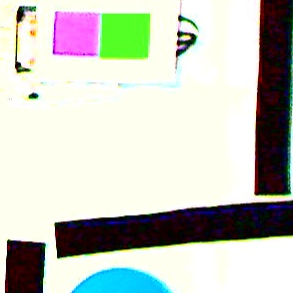
\includegraphics[width=\columnwidth]{pictures/colourmask1.png}
        \end{subfigure}
        \begin{subfigure}[t]{0.45\columnwidth}
        \centering
        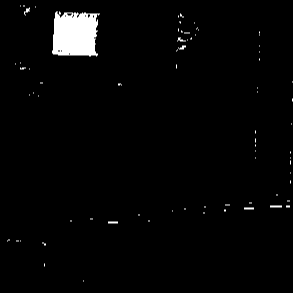
\includegraphics[width=\columnwidth]{pictures/colourmask2.png}
        \end{subfigure}
        \caption{\small Section of input image and corresponding colour mask for the purple robot marker.}
        \label{fig:colourmask}
\end{figure}

\subsubsection{Colour Masking Algorithm}

\begin{samepage}

To create a colour mask of a certain object type $o$ in a given image $P$ consisting of pixels with colours $p_i$, the average colour $\overline{C_o}$ and threshold value $T_o$ of the object type are retrieved. The mask $M$ then is an image of the same size and shape as $P$, with pixels of colours $m_i$, where
\nopagebreak
\[
m_i =
        \begin{cases}
        1 & \mbox{if } \dist( \overline{C_o}, p_i, ) < T_o \cdot \mu \\
        0 & \mbox{otherwise}
        \end{cases}
\]

\end{samepage}

$\mu$ here is what's known as the 'threshold multiplier', a constant value that allows for more or less leniency when matching colours. $\mu = 2$ would mean that the distance of a colour to the average may be twice as large as the distance found during calibration, and still be masked as belonging to the object type. Through experimentation we settled on $\mu = 1.5$.

\subsubsection{Optimization}
Although this report avoids code-specific details, special efforts went into optimizing the colour masking function, which are worth pointing out. This function needed to be quite fast, as it needs to run each frame, for all object types, over all pixels in the input stream. There were several optimizations made to aid in this.

First, as much of the required information is declared and initialized before the pixels are looped over, so that it need not be extracted over and over for each pixel.

Then, there is an 'early-out' mechanism, based on the fact that colour distance is the sum of the component distances. If a single component's distance (or the sum of two components' distances) is larger than the allowed colour distance, it is clear that the total distance is too large.

Since calculation of the absolute value of a number is used in the repeated colour distance calculation, it is an intensively used function and should be as fast as possible. Because colour component values can be represented by 8 bits, we implemented an absolute value function that works with 16-bit 'short integer' variables rather than the existing 32-bit function. We use a function invented and patented by Volkonsky in 1997 \cite{volkonsky2000apparatus}.

Finally, we utilize the .NET Parallel class to parallelize the loops over pixels and object type. This creates threads for each iteration of the different loops, causing the many iterations to be executed mostly simultaneously. This means that not all operations may be executed in order, but in our case this causes no problems, as pixels and object types are evaluated independently from each other.

\subsection{Contour Detection}
To be able to match an object in an image, we need to find a representation of the image such that we can assess whether it matches our ideas about the object. We do this by taking the masks created in the previous step, and converting them to polygons; vector representations of the contours of the masks. Thanks to EmguCV, this takes only a single line of code. An example of detected contours can be seen in \fref{fig:retrievedContours}.

\begin{figure}[h]
        \centering
        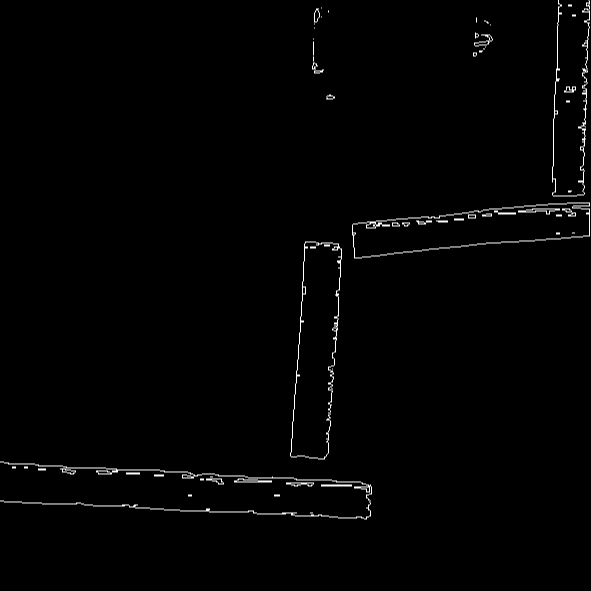
\includegraphics[width=\columnwidth]{pictures/retrievedContours.png}
        \caption{\small Example of retrieved wall contours.}
        \label{fig:retrievedContours}
\end{figure}

\subsection{Object Matching}
Having retrieved contours describing the matched shapes in the previous step, we now need to find out which contours actually correspond to the objects we are looking for, and which are flukes caused by fluctuating physical conditions. To do this, we try to match the contours to our ideas about the object types we are looking for.

Since we know which from which object type a particular set of contours was retrieved, we can look at contours to find specific properties that match our idea about the object type. If a contour matches the properties of the object type we are looking for, we accept it as being of that object type. Most contours we find are discarded as they are found not to match the object type. An example of matched objects can be see in \fref{fig:matchedObjects}.

\begin{figure}[h]
        \centering
        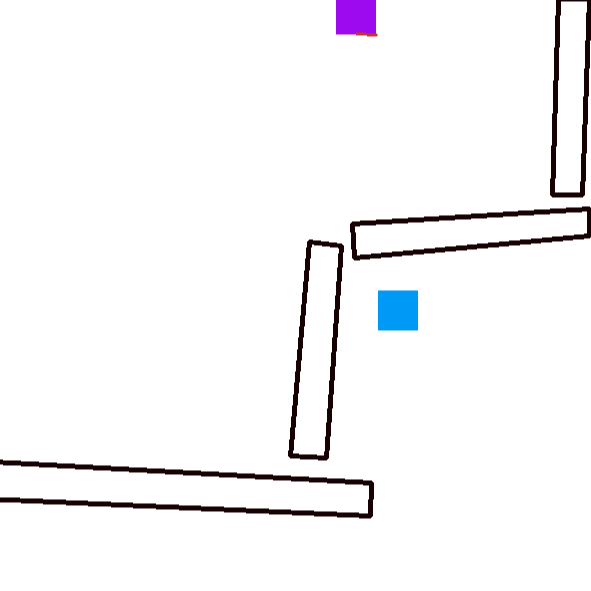
\includegraphics[width=\columnwidth]{pictures/matchedObjects.png}
        \caption{\small Objects matched from contours including those in \fref{fig:retrievedContours}.}
        \label{fig:matchedObjects}
\end{figure}

There are practically two different ways of matching contours to object types: rectangles and arbitrary shapes.

\subsubsection{Matching Rectangles}
\label{sec:matchingRectangles}
Many of the object types we are looking for are rectangular in shape. To check whether a particular contour is rectangular, we start by computing the convex hull of the contour. We do this because we know rectangles are convex, and any shape that matches our idea of a rectangle will be convex.

The points that make up the convex hull are then consolidated. By this we mean that points that are within a certain distance from each other are merged, and points that form an angle close to 180\degree with their neighbours are removed. Both of these modifications serve to clean up points that add little definition to the shape. An example of the consolidation process can be seen in \fref{fig:hullConsolidation}.

\begin{figure}[h]
        \centering
        \begin{subfigure}[t]{0.45\columnwidth}
        \centering
        
\includegraphics[width=\columnwidth]{pictures/hullConsolidation1.png}
        \end{subfigure}
        \begin{subfigure}[t]{0.45\columnwidth}
        \centering
        
\includegraphics[width=\columnwidth]{pictures/hullConsolidation2.png}
        \end{subfigure}
        \caption{A convex hull and its consolidated counterpart.}
        \label{fig:hullConsolidation}
\end{figure}

We then check whether the resulting shape has at least four points. We also check whether the area of the hull is above a certain value, thereby ignoring tiny variations in light and surface colour.

If these are true, we accept the contour as being close enough to rectangular in shape, and as being an instance of the particular object type we are looking for. 

\subsubsection{Matching Arbitrary Shapes}
If an object type's shape is not rectangular, then it is arbitrary (walls and the goal). Arbitrary shapes are matched by simplifying the contour (EmguCV functionality) and checking whether the contour has an area above a certain value (again, hereby ignoring small mistakes in the mask). If so, the contour is accepted as the object type in question.

\subsubsection{Matching Robots}
Since the robot has two distinct square on it that are aligned with its orientation, we can find the orientation of the robot as a vector from the first square through the second square. We also use the point between the squares to determine the position of the robot. We move this point somewhat along the orientation vector, such that it aligns with the centre of orientation of the robot (between the two motorized wheels). This procedure is visualized in \fref{fig:matchingRobots}.

\begin{figure}[h]
        \centering
        \begin{tikzpicture}[thick,scale=0.8, every node/.style={scale=1.6}]

\tikzset{cross/.style={thick, cross out, line width=4, minimum size=10pt, inner sep=0pt, outer sep=0pt},
%default radius will be 1pt. 
cross/.default={1pt}}

\begin{scope}[thick, rotate=-15]

\draw [gray,fill=lightgray] (-3.5,2) -- (3.5,2) -- (3.5,-2) -- (-3.5,-2) -- cycle;

\draw [green,fill=green!60!white,shift={(1.5,0)}] (1,1) -- (1,-1) -- (-1,-1) -- (-1,1) -- cycle;
\draw [yellow,fill=yellow!60!white,shift={(-1.5,0)}] (1,1) -- (1,-1) -- (-1,-1) -- (-1,1) -- cycle;

\draw [arrows=->,purple,line width=4pt,line cap=round] (1.5,0) -- (-6,0);

\draw (0,0) node[draw=white,cross,line cap=round] {};

\draw (1.5,0) circle(4pt);

\draw (-1.5,0) circle(4pt);

\draw (-3,0) node[draw=black,cross,line cap=round] {};

\draw [darkgray,fill=gray,shift={(-3,2.25)}] (-0.5,0.25) -- (0.5,0.25) -- (0.5,-0.25) -- (-0.5,-0.25) -- cycle;]

\draw [darkgray,fill=gray,shift={(-3,-2.25)}] (-0.5,0.25) -- (0.5,0.25) -- (0.5,-0.25) -- (-0.5,-0.25) -- cycle;]

\end{scope} 	

\end{tikzpicture}
        \caption{\small Visualization of the robot-matching process, with the robot marker in green, the transport robot marker in yellow, the center of those the white cross, the direction of the robot shown by the arrow, and the actual center of rotation the black cross. Light grey is the robot body, with the motorized wheels in dark grey.}
        \label{fig:matchingRobots}
\end{figure}

\subsection{Navigation Mesh}
Now that we have complete knowledge of all relevant objects in the world, including the location of the robot and the goal and the shapes of the walls, we can start thinking about how the robot is going to reach the goal. It seems obvious that we will need to use some kind of pathfinding algorithm.

\subsubsection{Initial Idea: Grid}
At first, we considered dividing the world up into a grid, with each grid tile either inside a wall or not inside a wall, then using the standard algorithm of pathfinding through this grid using A*. However, we foresaw several potential problems with this approach. For starters, to determine which points were inside walls, they would each need to be checked for inclusion in all wall objects. Likely a time-consuming task, especially since the number of tiles would need to be quite large in order to ensure a sufficiently high resolution. Such a resolution would be needed to allow for smaller passages through obstacles to be captured. Also, a grid-based pathing approach would limit us to movement in horizontal, vertical and diagonal directions, or require us to find tricks to expand those directions. Finally, running A* on such a large amount of points would probably be another performance issue.

\subsubsection{NavMesh Definition}
We found an alternative in navigation meshes (or navmeshes): a technique gleaned from use in video game AI. The core concept of navigation meshes is to divide the world up into interconnected areas of arbitrary shape, forming a network. That network can then be used to perform the (initial) steps of pathfinding on, for example A*. An example of such a mesh can be seen in \fref{fig:navmeshExample}.

\begin{figure}[h]
        \centering
        \begin{tikzpicture}[thick,scale=1, every node/.style={scale=0.8}]

\begin{scope}

\clip (0,0) -- (8,0) -- (8,-6) -- (0,-6) -- cycle;

\draw [line width=0,fill=yellow!15!white] (0,0) -- (8,0) -- (8,-6) -- (0,-6) -- cycle;

\draw [green!60!white,line width=2,line cap=round] (3,0) -- (6,-1);

\draw [green!60!white,line width=2,line cap=round] (5,-4) -- (6,-2);

\draw [green!60!white,line width=2,line cap=round] (2,-3) -- (0,-6);

\draw [green!60!white,line width=2,line cap=round] (3,-3) -- (4,-4);

\draw [green!60!white,line width=2,line cap=round] (4,-5) -- (0,-6);

\draw [green!60!white,line width=2,line cap=round] (5,-5) -- (8,-6);

\draw [fill=black,rounded corners=1] (2,0) -- (3,0) -- (3,-3) -- (2,-3) -- cycle;

\draw [fill=black,rounded corners=1] (6,-1) -- (8,-1) -- (8,-2) -- (6,-2) -- cycle;

\draw [fill=black,rounded corners=1] (4,-4) -- (5,-4) -- (5,-5) -- (4,-5) -- cycle;

\end{scope}

\draw [line width=2,rounded corners=1] (0,0) -- (8,0) -- (8,-6) -- (0,-6) -- cycle;

\end{tikzpicture}
        \caption{\small Generic example of a navmesh with walls in black, navigation area boundaries in green.}
        \label{fig:navmeshExample}
\end{figure}

For our specific case, we decided to add several constraints to the navmesh geometry. Most importantly, all individual areas in the navmesh  are convex shapes. This ensures that when the robot is in a particular area, it can always move freely to any other point in the area. Effectively, this means that the only pathfinding we need to do is between the edges that connect areas, as all movement between those is unobstructed. This does not however take into account the width of the vehicle as it moves close to the edge of an area, which is discussed in \sref{sec:pathrefinement}.

\subsubsection{Construction}
There are several steps involved in the construction of the navmesh. First, the negative space left by the walls is triangulated. The triangles are then consolidated into a network of polygons. Finally, the small-passage-avoidance algorithm ensures that narrow passages are removed from the network.

\paragraph{Triangulation}
In order to start building the navmesh, we triangulate the negative space left by the wall objects. Technically, we create a large polygon that covers the whole world, and then add the walls into that polygon as holes. Triangulating that polygon using Triangle.NET results in what can be seen as a rough version of the navmesh. Although the triangles could already at this point be used for pathfinding, the network that they form is unnecessarily large. An example of negative space triangulation can be seen in \fref{fig:triangulation}.

\begin{figure}[h]
        \centering
        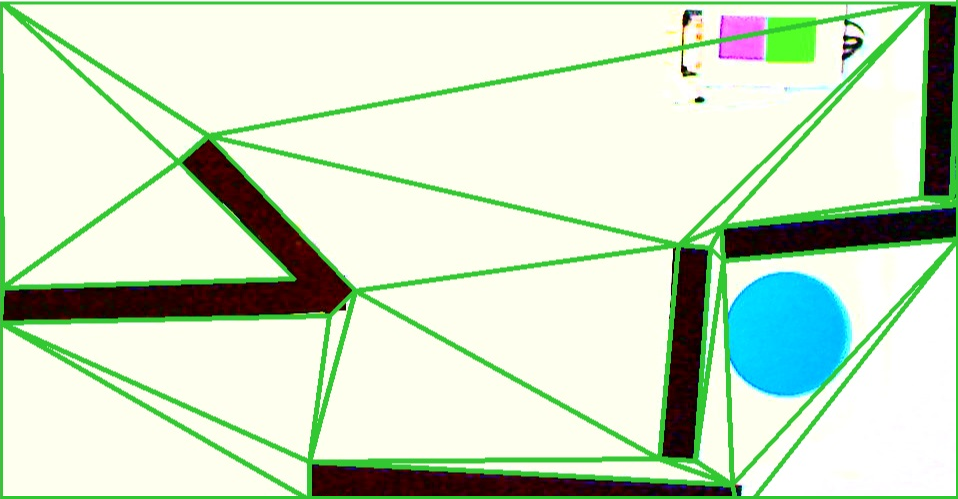
\includegraphics[width=\columnwidth]{pictures/triangulation.png}
        \caption{\small The negative space around some walls, triangulated.}
        \label{fig:triangulation}
\end{figure}

\paragraph{Consolidation}
We now start merging neighbouring triangles into larger polygons using a process we call consolidation (not to be confused with intra-polygon consolidation discussed in \sref{sec:matchingRectangles}). When two polygons are merged, they form a new polygon with the same shape as the two initial polygons combined. This new polygon takes the place of the two initial polygons in the network. An visualization of polygon consolidation can be seen in \fref{fig:consolidation}.

\begin{figure}[h]
        \centering
        \begin{subfigure}[t]{0.45\columnwidth}
        \centering
        \begin{tikzpicture}[thick,scale=1, every node/.style={scale=1}]

\draw [line width=2,line cap=round,fill=yellow!15!white] (3,0) -- (6,-1) -- (6,-2) -- (5,-4) -- (4,-4)  -- (3,-3)-- cycle;

\draw [line width=2,line cap=round,fill=yellow!15!white] (3,0) -- (5,-4);

\end{tikzpicture}
        \end{subfigure}
        \begin{subfigure}[t]{0.45\columnwidth}
        \centering
        \begin{tikzpicture}[thick,scale=1, every node/.style={scale=1}]

\draw [line width=2,line cap=round,fill=yellow!15!white] (3,0) -- (6,-1) -- (6,-2) -- (5,-4) -- (4,-4)  -- (3,-3)-- cycle;

\end{tikzpicture}
        \end{subfigure}
        \caption{\small A pair of polygons on the left and their consolidated version on the right. All of these polygons are convex.}
        \label{fig:consolidation}
\end{figure}

To decide which polygons to merge, all combinations between two neighbouring polygons are evaluated. If the polygons would form a convex shape when merged, then so they should be.

There is the important question of the order in which to merge polygons, since the merger of polygons $A$ and $B$ will exclude the merger of polygons $B$ and $C$. Since the aim is to create as few and as large areas as possible, the policy is to check out smaller polygons first. Since we don't want to use two smaller polygons to create a new small area with no consolidable neighbours, the policy is to look for consolidations with larger neighbours first. These policies make for a navmesh with mostly large areas.

This process of consolidation is executed iteratively. That is, consolidated polygons are again checked for new consolidation possibilities. When no more valid combinations can be found, consolidation is completed. An example of the result of the consolidation process can be seen in \fref{fig:consolidatedTriangles}.

\begin{figure}[h]
        \centering
        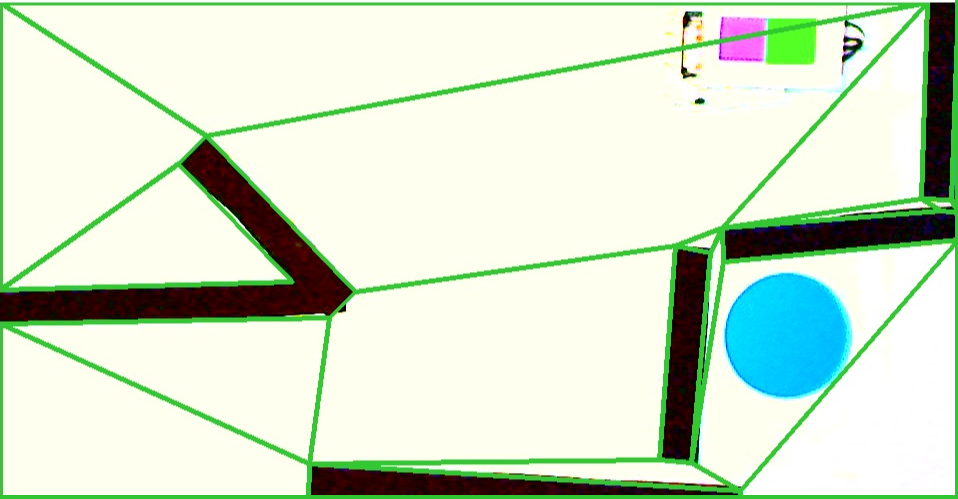
\includegraphics[width=\columnwidth]{pictures/consolidatedTriangles.png}
        \caption{\small The triangles from \fref{fig:triangulation}, consolidated into polygons.}
        \label{fig:consolidatedTriangles}
\end{figure}

\paragraph{Avoiding small passages}
Since our robot is not a point and has dimensions, we want to avoid producing a path between two walls that the robot would not physically be able to fit through. Given the workings of our navmesh, all edges that connect two areas start and end on walls (specifically, corners of walls). This makes for an easy way to approach the problem of small passage avoidance. Still, finding a method that worked correctly in all situations was a challenge.

Perhaps the most obvious thing to do in order to find connections between areas that are too small to pass through is to check whether the edge that connects the areas is longer than the width of the vehicle. This turns out to work fine in some cases, but not in others, especially when the edge is at a large angle with neighbouring edges. This is demonstrated in \fref{fig:edgeLengthMethod}.

\begin{figure}[h]
        \centering
        \begin{subfigure}[t]{0.45\columnwidth}
        \centering
        \begin{tikzpicture}[thick,scale=.5, every node/.style={scale=1}]

\begin{scope}

\clip (-1,0) -- (5,0) -- (5,8) -- (-1,8) -- cycle;

\draw [line width=0,fill=yellow!15!white] (-1,0) -- (5,0) -- (5,8) -- (-1,8) -- cycle;

\draw [red!60!white,line width=2,line cap=round] (2.5,3.5) -- (2.5,4.5);
\draw [red!60!white,line width=2,line cap=round] (3.5,3.5) -- (3.5,4.5);

\draw [fill=black,rounded corners=1] (1,0) -- (2.5,3.5) -- (3.5,3.5) -- (5,0) -- cycle;
\draw [fill=black,rounded corners=1] (1,8) -- (2.5,4.5) -- (3.5,4.5) -- (5,8) -- cycle;

\draw [green,fill=green!60!white,rounded corners=1] (-3,3) -- (-3,5) -- (0,5) -- (0,3) -- cycle;

\draw [arrows=|<->|,purple,line width=1pt,line cap=round] (0.5,5) -- (0.5,3);
\draw [arrows=|<->|,purple,line width=1pt,line cap=round] (2,4.5) -- (2,3.5);

\end{scope}

\draw [line width=2,rounded corners=1] (-1,0) -- (5,0) -- (5,8) -- (-1,8) -- cycle;

\end{tikzpicture}
        \subcaption{\small Edge-length method working correctly (robot in green, walls in black, avoided edges in red)}
        \end{subfigure}
        \begin{subfigure}[t]{0.45\columnwidth}
        \centering
        \begin{tikzpicture}[thick,scale=.5, every node/.style={scale=1}]

\begin{scope}

\clip (0,0) -- (6,0) -- (6,8) -- (0,8) -- cycle;

\draw [line width=0,fill=yellow!15!white] (0,0) -- (6,0) -- (6,8) -- (0,8) -- cycle;

\draw [blue!60!white,line width=2,line cap=round] (4,7) -- (3,4.5);
\draw [blue!60!white,line width=2,line cap=round] (4,1) -- (3,3.5);

\draw [fill=black,rounded corners=1] (4,7) -- (6,7) -- (6,1) -- (4,1) -- cycle;
\draw [fill=black,rounded corners=1] (0,4.5) -- (3,4.5) -- (3,3.5) -- (0,3.5) -- cycle;

\draw [fill=green!60!white,rounded corners=1,shift={(1,2.25)}] (-3,3) -- (-3,5) -- (0,5) -- (0,3) -- cycle;

\draw [arrows=|<->|,purple,line width=1pt,line cap=round,shift={(1,2.25)}] (0.5,5) -- (0.5,3);
\draw [arrows=|<->|,purple,line width=1pt,line cap=round] (3.33,7.33) -- (2.33,4.88);

\end{scope}

\draw [line width=2,rounded corners=1] (0,0) -- (6,0) -- (6,8) -- (0,8) -- cycle;

\end{tikzpicture}
        \subcaption{\small Edge-length method working incorrectly: the edges are not avoided even though the passage is too narrow.}
        \end{subfigure}
        \caption{\small Edge-length method of avoiding small passages.}
        \label{fig:edgeLengthMethod}
\end{figure}

When confronted with the previous problem, we were quick to suggest that a solution might be to evaluate the size of the whole polygon -- looking at some measurement of its width to determine whether the robot would be able to fit through it. This would solve the above problem, but would falsely identify some other polygons as being too narrow, as can be seen in \fref{fig:polygonWidthMethod}.

\begin{figure}[h]
        \centering
        \begin{tikzpicture}[thick,scale=1, every node/.style={scale=1}]

\begin{scope}

\clip (0,0) -- (6,0) -- (6,6) -- (0,6) -- cycle;

\draw [line width=0,fill=yellow!15!white] (0,0) -- (6,0) -- (6,6) -- (0,6) -- cycle;

\draw [red!60!white,line width=4,line cap=round] (3.5,1) -- (3.5,5);
\draw [red!60!white,line width=4,line cap=round] (4.5,5) -- (4.5,1);
\draw [red!60!white,line width=4,line cap=round] (3.5,1) -- (4.5,1);

\draw [fill=black,rounded corners=1] (0,0) -- (0,1) -- (3.5,1) -- (3.5,0) -- cycle;
\draw [fill=black,rounded corners=1] (4.5,0) -- (4.5,1) -- (8,1) -- (8,0) -- cycle;
\draw [fill=black,rounded corners=1] (3.5,5) -- (3.5,6) -- (4.5,6) -- (4.5,5) -- cycle;

\draw [fill=green!60!white,rounded corners=1,shift={(1,-0.75)}] (-3,3) -- (-3,5) -- (0,5) -- (0,3) -- cycle;

\draw [arrows=|<->|,purple,line width=2pt,line cap=round,shift={(1,-0.75)}] (0.5,5) -- (0.5,3);
\draw [arrows=|<->|,purple,line width=2pt,line cap=round] (3.5,3) -- (4.5,3);

\end{scope}

\draw [line width=2,rounded corners=1] (0,0) -- (6,0) -- (6,6) -- (0,6) -- cycle;

\end{tikzpicture}
        \caption{\small A polygon incorrectly identified as impassable by the width-based method.}
        \label{fig:polygonWidthMethod}
\end{figure}

\begin{samepage}

After some more considerations, we found a reliable method $A_e$ of determining whether an edge $e$ connecting two areas should be avoided due to it being too small to pass through.\textsf{}
\begin{align*}
A_e = &\ \forall p,q \in P_e, \exists f \in E_q : \\
&\ p \neq q \land e \neq f \land \dist(p,\proj(p,e)) < \psi
\end{align*}
\nopagebreak
where
\begin{align*}
P_e &= \textrm{the set of points defining edge $e$} \\
E_p &= \textrm{the set of edges partially defined by point $p$} \\
\proj(p,e) &= \textrm{the projection of point $p$ onto edge $e$} \\
\dist(p,q) &= \textrm{the distance between two points $p$ and $q$} \\
\psi &= \textrm{the width of the robot}
\end{align*}

\end{samepage}

In words: an edge must be avoided if, for both points that define the edge, there exists another edge connected to the other point, such that the distance of the projection of the point onto that edge is smaller than the width of the robot. A visualization of this function is shown in \fref{fig:projectionMethod}.

\begin{figure}[h]
        \centering
        \begin{subfigure}[t]{0.45\columnwidth}
        \centering
        \begin{tikzpicture}[thick,scale=.5, every node/.style={scale=1}]

\begin{scope}

\clip (-1,0) -- (5,0) -- (5,8) -- (-1,8) -- cycle;

\draw [line width=0,fill=yellow!15!white] (-1,0) -- (5,0) -- (5,8) -- (-1,8) -- cycle;

\draw [green!60!white,line width=2,line cap=round] (2.5,3.5) -- (2.5,4.5);
\draw [black!60!white,line width=2,line cap=round] (3.5,3.5) -- (3.5,4.5);

\draw [fill=black,rounded corners=1] (1,0) -- (2.5,3.5) -- (3.5,3.5) -- (5,0) -- cycle;
\draw [fill=black,rounded corners=1] (1,8) -- (2.5,4.5) -- (3.5,4.5) -- (5,8) -- cycle;

\draw [fill=green!60!white,rounded corners=1] (-3,3) -- (-3,5) -- (0,5) -- (0,3) -- cycle;

\draw [blue!60!white,line width=2,line cap=round] (2.5,3.5) -- (3.5,3.5);
\draw [arrows=->,red!50!blue,line width=1pt,line cap=round] (2.5,4.5) -- (2.5,3.5);
\draw [red!50!blue,fill=red!50!blue] (2.5,4.5) circle (4pt);

\draw [arrows=|<->|,purple,line width=1pt,line cap=round] (0.5,5) -- (0.5,3);
\draw [arrows=|<->|,purple,line width=1pt,line cap=round] (2,4.5) -- (2,3.5);

\end{scope}

\draw [line width=2,rounded corners=1] (-1,0) -- (5,0) -- (5,8) -- (-1,8) -- cycle;

\end{tikzpicture}
        \subcaption{\small }
        \end{subfigure}
        \begin{subfigure}[t]{0.45\columnwidth}
        \centering
        \begin{tikzpicture}[thick,scale=.5, every node/.style={scale=1}]

\begin{scope}

\clip (0,0) -- (6,0) -- (6,8) -- (0,8) -- cycle;

\draw [line width=0,fill=yellow!15!white] (0,0) -- (6,0) -- (6,8) -- (0,8) -- cycle;

\draw [green!60!white,line width=2,line cap=round] (4,7) -- (3,4.5);
\draw [black!60!white,line width=2,line cap=round] (4,1) -- (3,3.5);

\draw [fill=black,rounded corners=1] (4,7) -- (6,7) -- (6,1) -- (4,1) -- cycle;
\draw [fill=black,rounded corners=1] (0,4.5) -- (3,4.5) -- (3,3.5) -- (0,3.5) -- cycle;

\draw [green,fill=green!60!white,rounded corners=1,shift={(1,2.25)}] (-3,3) -- (-3,5) -- (0,5) -- (0,3) -- cycle;

\draw [blue!60!white,line width=2,line cap=round] (4,1) -- (4,7);
\draw [arrows=->,red!50!blue,line width=1pt,line cap=round] (3,4.5) -- (4,4.5);
\draw [red!50!blue,fill=red!50!blue] (3,4.5) circle (4pt);

\draw [arrows=|<->|,purple,line width=1pt,line cap=round,shift={(1,2.25)}] (0.5,5) -- (0.5,3);
\draw [arrows=|<->|,purple,line width=1pt,line cap=round]  (3,5) -- (4,5);

\end{scope}

\draw [line width=2,rounded corners=1] (0,0) -- (6,0) -- (6,8) -- (0,8) -- cycle;

\end{tikzpicture}
        \subcaption{\small }
        \end{subfigure}
        \begin{subfigure}[t]{0.45\columnwidth}
        \centering
        \begin{tikzpicture}[thick,scale=0.5, every node/.style={scale=0.5}]

\begin{scope}

\clip (0,0) -- (6,0) -- (6,6) -- (0,6) -- cycle;

\draw [line width=0,fill=yellow!15!white] (0,0) -- (6,0) -- (6,6) -- (0,6) -- cycle;

\draw [black!60!white,line width=2,line cap=round] (3.5,1) -- (3.5,5);
\draw [black!60!white,line width=2,line cap=round] (4.5,5) -- (4.5,1);
\draw [green!60!white,line width=2,line cap=round] (3.5,1) -- (4.5,1);

\draw [fill=black,rounded corners=1] (0,0) -- (0,1) -- (3.5,1) -- (3.5,0) -- cycle;
\draw [fill=black,rounded corners=1] (4.5,0) -- (4.5,1) -- (8,1) -- (8,0) -- cycle;
\draw [fill=black,rounded corners=1] (3.5,5) -- (3.5,6) -- (4.5,6) -- (4.5,5) -- cycle;

\draw [green,fill=green!60!white,rounded corners=1,shift={(1,-0.75)}] (-3,3) -- (-3,5) -- (0,5) -- (0,3) -- cycle;

\draw [blue!60!white,line width=2,line cap=round] (4.5,1) -- (4.5,5);
\draw [arrows=->,red!50!blue,line width=1pt,line cap=round] (3.5,1) -- (4.5,1);
\draw [red!50!blue,fill=red!50!blue] (3.5,1) circle (4pt);

\draw [arrows=|<->|,purple,line width=1pt,line cap=round,shift={(1,-0.75)}] (0.5,5) -- (0.5,3);
\draw [arrows=|<->|,purple,line width=1pt,line cap=round] (3.5,1.5) -- (4.5,1.5);

\end{scope}

\draw [line width=2,rounded corners=1] (0,0) -- (6,0) -- (6,6) -- (0,6) -- cycle;

\end{tikzpicture}
        \subcaption\small {}
        \end{subfigure}
        \begin{subfigure}[t]{0.45\columnwidth}
        \centering
        \begin{tikzpicture}[thick,scale=0.5, every node/.style={scale=0.5}]

\begin{scope}

\clip (0,0) -- (6,0) -- (6,6) -- (0,6) -- cycle;

\draw [line width=0,fill=yellow!15!white] (0,0) -- (6,0) -- (6,6) -- (0,6) -- cycle;

\draw [green!60!white,line width=2,line cap=round] (3.5,1) -- (3.5,5);
\draw [black!60!white,line width=2,line cap=round] (4.5,5) -- (4.5,1);
\draw [black!60!white,line width=2,line cap=round] (3.5,1) -- (4.5,1);

\draw [fill=black,rounded corners=1] (0,0) -- (0,1) -- (3.5,1) -- (3.5,0) -- cycle;
\draw [fill=black,rounded corners=1] (4.5,0) -- (4.5,1) -- (8,1) -- (8,0) -- cycle;
\draw [fill=black,rounded corners=1] (3.5,5) -- (3.5,6) -- (4.5,6) -- (4.5,5) -- cycle;

\draw [green,fill=green!60!white,rounded corners=1,shift={(1,-0.75)}] (-3,3) -- (-3,5) -- (0,5) -- (0,3) -- cycle;

\draw [blue!60!white,line width=2,line cap=round] (4.5,1) -- (3.5,1);
\draw [arrows=->,red!50!blue,line width=1pt,line cap=round] (3.5,5) -- (3.5,1) ;
\draw [red!50!blue,fill=red!50!blue] (3.5,5) circle (4pt);

\draw [arrows=|<->|,purple,line width=1pt,line cap=round,shift={(1,-0.75)}] (0.5,5) -- (0.5,3);
\draw [arrows=|<->|,purple,line width=1pt,line cap=round] (4,5) -- (4,1);

\end{scope}

\draw [line width=2,rounded corners=1] (0,0) -- (6,0) -- (6,6) -- (0,6) -- cycle;

\end{tikzpicture}
        \subcaption{\small }
        \end{subfigure}
        \caption{\small Purple projection of one point on the green edge onto the neighbouring blue edge, solving all previously shown problems. In figures (a) through (c), the projection distance is smaller than the robot width, and the green edge is avoided. In figure (d), the opposite is true.}
        \label{fig:projectionMethod}
\end{figure}

This method is completely successful at determining whether edges should be avoided or not. When a narrow edge is found, the connectivity that it forms between two polygons is removed from the navmesh.

\subsection{Pathing}
With the navmesh area-network in place, we can find a path from the robot to the goal. After embedding the start and end points into the navmesh, A* is used to find a path between them, after which proximal points are removed from the path. The result of all this is a single point; the location that the robot presently needs to travel towards. The rest of the path is discarded, as we expect the world may change with time, rendering the previously computed path irrelevant. An example of a computed path can be found in \fref{fig:computedPath}.

\subsubsection{Embedding points}
We need to insert the start and end points of our desired path (the robot and goal locations) into the navmesh. To do this for either of those points, we find the polygon in the navmesh that contains the point. We then create connections between the point and the edges of that polygon. The result of this process can be seen in \fref{fig:finalNavMesh}.

\begin{figure}[h]
        \centering
        \begin{tikzpicture}[thick,scale=1, every node/.style={scale=0.8}]

\tikzset{cross/.style={thick, cross out, line width=4, minimum size=10pt, inner sep=0pt, outer sep=0pt},
%default radius will be 1pt. 
cross/.default={1pt}}

\begin{scope}

\clip (0,0) -- (8,0) -- (8,-6) -- (0,-6) -- cycle;

\draw [line width=0,fill=yellow!15!white] (0,0) -- (8,0) -- (8,-6) -- (0,-6) -- cycle;

\draw [black!60!white,line width=2,line cap=round] (3,0) -- (6,-1);
\draw [black!60!white,line width=2,line cap=round] (5,-4) -- (6,-2);
\draw [black!60!white,line width=2,line cap=round] (2,-3) -- (0,-6);
\draw [black!60!white,line width=2,line cap=round] (3,-3) -- (4,-4);
\draw [black!60!white,line width=2,line cap=round] (4,-5) -- (0,-6);
\draw [black!60!white,line width=2,line cap=round] (5,-5) -- (8,-6);

\draw [fill=black,rounded corners=1] (2,0) -- (3,0) -- (3,-3) -- (2,-3) -- cycle;
\draw [fill=black,rounded corners=1] (6,-1) -- (8,-1) -- (8,-2) -- (6,-2) -- cycle;
\draw [fill=black,rounded corners=1] (4,-4) -- (5,-4) -- (5,-5) -- (4,-5) -- cycle;

\draw [blue!60!white,line width=2,line cap=round,rounded corners=1] (4.5,-0.5) -- (5.5,-3) -- (6.5,-5.5)  -- (2,-5.5) -- (1,-4.5) -- (3.5,-3.5) -- cycle;
\draw [blue!60!white,line width=2,line cap=round,rounded corners=1] (2,-5.5) -- (3.5,-3.5) -- (5.5,-3);

\draw [blue!60!white,line width=2,line cap=round,rounded corners=1] (1,-1) -- (1,-4.5);
\draw (1,-1) node[draw=green,cross,line cap=round] {};

\draw [blue!60!white,line width=2,line cap=round] (5.5,-3) -- (7,-4) -- (6.5,-5.5);
\draw (7,-4) node[draw=red,cross,line cap=round] {};


\end{scope}

\draw [line width=2,rounded corners=1] (0,0) -- (8,0) -- (8,-6) -- (0,-6) -- cycle;

\end{tikzpicture}
        \caption{\small Start and end points embedded into navmesh, showing edges in grey and connections in blue.}
        \label{fig:finalNavMesh}
\end{figure}

\subsubsection{A* / Dijkstra}

Now that all the ingredients are in place, we run our implementation of A* to find a path from start to finish. It should be noted that we never bothered to implement a heuristic estimate function, since our search space is so small (thanks to the navmesh) that its contribution to performance would be negligible. Because of this, we are really just running Dijkstra's algorithm.

\begin{samepage}

A call to our A* implementation is structured as follows:
\nopagebreak
\[
\textrm{A*}(\alpha,\beta,N,D,H) = P
\]
\nopagebreak
where
\begin{align*}
\alpha =&\ \textrm{the start state} \\
\beta =&\ \textrm{the end state} \\
N =&\ \textrm{a function of the form $N(s)$} \\
&\ \textrm{to retrieve the child states of state $s$} \\
D =&\ \textrm{a function of the form $D(s,t)$} \\
&\ \textrm{to retrieve the cost of traversing from state $s$ to state $t$} \\
H =&\ \textrm{a function of the form $H(s)$} \\
&\ \textrm{to retrieve the heuristc estimate for state $s$} \\
P =&\ \textrm{a sequence of states that form the path}
\end{align*}

\end{samepage}

Any data type can be used to represent states by defining the above functions. In a (semi) functional language such as C\# this is easily achieved through the use of lambda expressions.

\subsubsection{Proximal node removal}
Having found the path we wish to travel, we will remove all nodes that the robot is currently close to from the front of the path. This way, we determine wether the robot has reached a point in a path. Otherwise, it would practically never reach the point, due to the continuous nature of the locations of the point and the robot. The function $\Pi$ to clean the path of proximal nodes can be written recursively.

\begin{samepage}

\[
\Pi(P) =
        \begin{cases}
        P & \textrm{if } \dist(R,P_0) > \Delta \\
        \Pi( P \setminus P_0 ) & \textrm{otherwise}
        \end{cases}
\]
\nopagebreak
where
\begin{align*}
P &= \textrm{a sequence of points that form the path} \\
\dist(p,q) &= \textrm{the distance between points $p$ and $q$} \\
R &= \textrm{the current location of the robot} \\
\Delta &= \textrm{distance at which robot is said to reach a point}
\end{align*}

\end{samepage}


What remains is a sequence of nodes starting with the first location the robot needs to move towards. This location is handed over to the robot control system.

\begin{figure}[h]
        \centering
        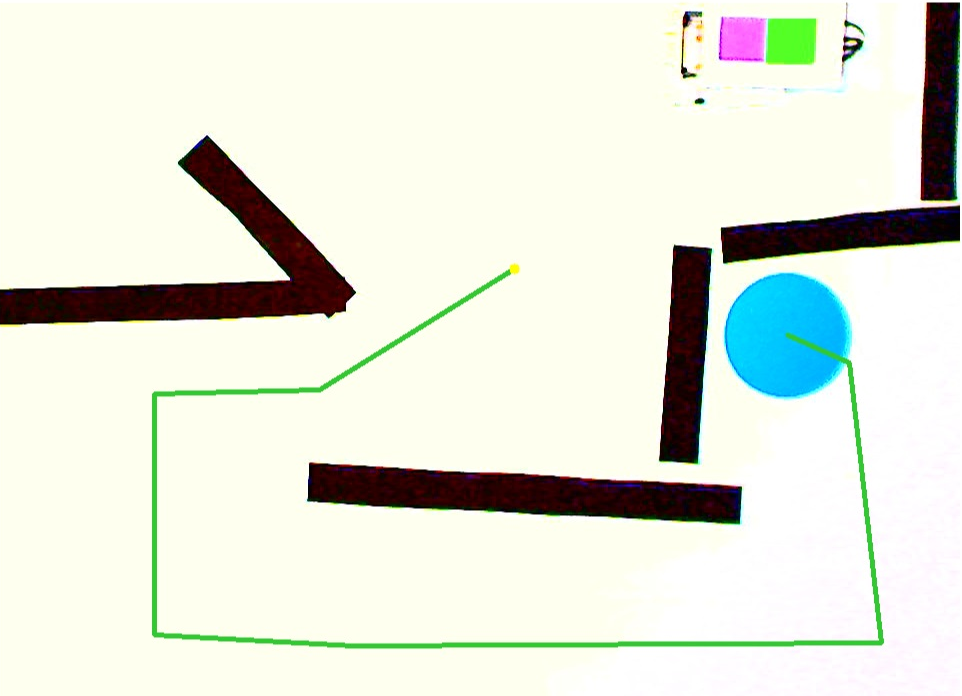
\includegraphics[width=\columnwidth]{pictures/computedPath.png}
        \caption{\small A path found through the navmesh from \fref{fig:consolidatedTriangles} (note: only partial navmesh shown in previous images). The yellow dot is the current point the robot should move towards.}
        \label{fig:computedPath}
\end{figure}

\subsection{Communication}
AForge.NET supplies various convenience methods to communicate with LEGO NXT Bricks through bluetooth. A serial port connection is established between the computer and the brick, and the framework converts high-level messages such as 'set motor A's speed to 50' to a correctly formatted bytestring. To tweak driving speed and manage robot connections, we created a small interface seen in \fref{fig:robotInterface}.

\begin{figure}[h]
		\centering
		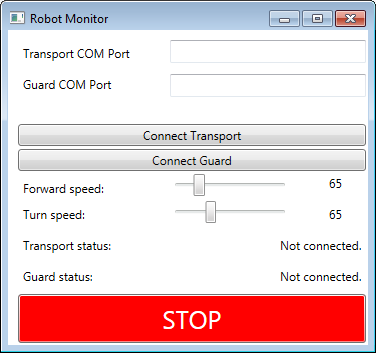
\includegraphics[width=\columnwidth]{pictures/robotInterface.png}
        \caption{\small Visual interface to connect with robots and manage speed.}
        \label{fig:robotInterface}
\end{figure}

\subsection{Control}

\begin{samepage}

Once we have established a connection between the computer and the robot, we can start executing the plan we created. In order to achieve this, we need to know a couple of things:
\nopagebreak
\begin{itemize}
        \item Robot's position
        \item Robot's orientation
        \item Desired position (first position to reach in the calculated path)
\end{itemize}

\end{samepage}

We find all of these in previous steps in our processing pipeline. Next, we define a couple of values (also see \fref{fig:controlAngles}):

\begin{description}
\item[Destination offset angle ($\delta_{dest}$)] The difference between the robot's orientation and the angle of the robot with the destination.
\item[Maximum offset margin ($\delta_{max}$)] The maximum offset with the destination that still passes as 'the correct direction'.
\end{description}

To decide what the robot will actually do (turn or drive forward), we compare these values. If $\delta_{dest} > \delta_{max}$, the robot turns according to the following:

\[
\textrm{direction} =
\begin{cases}
\textrm{left} & \textrm{if } \delta_{dest} < 0 \\
\textrm{right} & \textrm{otherwise}
\end{cases}
\]

We added some flexibility in our code to avoid the robot flipping from left to right constantly when $\lvert \delta_{dest}\rvert$ is close to $180\degree$.
If $\delta_{dest} \leq \delta_{max}$ it's easy; we just have the robot drive forward.

\begin{figure}[h]
        \centering
        \begin{tikzpicture}[thick,scale=0.6, every node/.style={scale=1.6}]

\tikzset{cross/.style={thick, cross out, line width=4, minimum size=10pt, inner sep=0pt, outer sep=0pt},
%default radius will be 1pt. 
cross/.default={1pt}}

\newcommand{\goalrotation}{-110}
\newcommand{\dmax}{15}
\newcommand{\ddestradius}{1}
\newcommand{\globalrotation}{30}

\newcommand{\extratextradius}{0.5}
\newcommand{\goaldistance}{6}
\newcommand{\conedistance}{8}

\begin{scope}[thick,rotate=\globalrotation]

\draw [gray,fill=lightgray] (-6.5,2) -- (0.5,2) -- (0.5,-2) -- (-6.5,-2) -- cycle;
\draw [darkgray,fill=gray] (-0.5,2.5) -- (0.5,2.5) -- (0.5,2) -- (-0.5,2) -- cycle;]
\draw [darkgray,fill=gray] (-0.5,-2.5) -- (0.5,-2.5) -- (0.5,-2) -- (-0.5,-2) -- cycle;]

\draw [yellow,fill=yellow!60!white,shift={(-1.5,0)}] (-1,1) -- (1,1) -- (1,-1) -- (-1,-1) -- cycle;
\draw [green,fill=green!60!white,shift={(-4.5,0)}] (-1,1) -- (1,1) -- (1,-1) -- (-1,-1) -- cycle;

\draw [line width=2,yellow,fill=yellow,fill opacity=0.2,rounded corners=1ex] (0,0) ++(\goalrotation-\dmax:\conedistance) -- (0,0) -- (\goalrotation+\dmax:\conedistance);

\draw (0,0) ++(\goalrotation:\conedistance-\extratextradius) node [rotate=\goalrotation+90+\globalrotation]{\small $\delta_{max}$};

\draw [line width=2] (0,0) ++(0:\ddestradius) arc (0:\goalrotation:\ddestradius);

\draw (0,0) ++(\goalrotation/2:\ddestradius+\extratextradius) node [rotate=\goalrotation/2+90+\globalrotation]{\small $\delta_{dest}$};

\draw [arrows=->,purple,line width=4pt,line cap=round] (0,0) -- (4,0);

\begin{scope}[rotate=\goalrotation]

\draw [cyan,fill=cyan!60!white] (\goaldistance,0) circle(20pt);
\draw [arrows=->,blue,line width=4pt,line cap=round] (0,0) -- (\goaldistance,0);

\end{scope}

\end{scope}

\end{tikzpicture}
        \caption{\small Visual representation of the information used to determine the movement of the robot.}
        \label{fig:controlAngles}
\end{figure}

\subsection{Robustness}
In each of the previous steps, we have always assumed that certain information was present. For example, we assumed that a path was possible between the robot and the goal, while this may not always be the case, depending on the layout of the walls. This may raise the question of what happens in such cases. In fact, when the program encounters such a problem, or even an exception raised at some point in the code, the current run through the analysis pipeline is aborted and the program waits for a new input image to arrive.

At such a time, the robot simply continues executing the last action it received from the analysis pipeline. The assumption being that some subsequent input image will have different conditions such that the analysis pipeline is once again able to run fully, resulting in updated information. This approach might seem dangerous, but actually works out quite well, providing that the user knows about certain restrictions when manipulating the world (such as the need for there to be a path to the goal).

\section{Physical Considerations}
We encountered several problems related to the physical objects involved in our project that caused us to take certain decisions. Please note that the team member responsible for building the robots and the world was somehow unable to write about his work. Thus, we cannot write about the decisions taken in the design of the robot and most of the world. There were several large issues that we will discuss, however.

\subsection{Calibration Sheets}
We need the program to recognize a certain colour in all locations on the playing field, under slightly varying light conditions. To achieve this, we use calibration sheets during the colour calibration phase. These A4-sized sheets contain samples of all the colours that are relevant to our program. We place these sheets in different areas such that they are all in different light conditions. We then calibrate using the colours on these sheets (as well as any other instances of the associated object type that happen to be on the field). This gives our program a good grasp of the range of colours that a particular object type can be perceived as.

\subsection{Light}
Although we use a calibration system that is able to largely cope with differences in light conditions across the playing field, it cannot cope as well with differences in light conditions between points in time. An example of this inability occurring might be during demonstrations, when many people are moving close to the playing field, casting moving shadows.

In order to diminish the effect of shadows, we decided to suspend a very bright lamp from the ceiling, right above the playing field. The light ensures that shadows cast by people do not appear on the field. A photo of the lamp suspended from the ceiling can be seen in \fref{fig:photo2light}.

\begin{figure}[h]
	\centering
	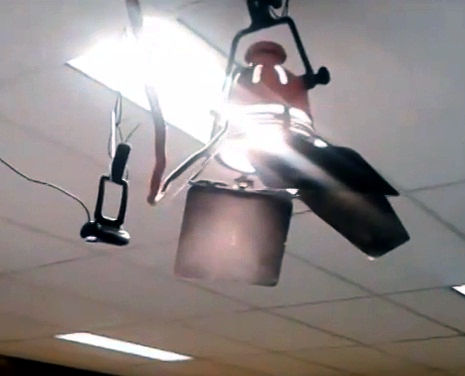
\includegraphics[width=\columnwidth]{pictures/photo2light.png}
	\caption{\small The camera and the lamp hanging from the ceiling above the playing field.}
	\label{fig:photo2light}
\end{figure}

\subsection{Covering with White}
We experienced major difficulties in trying to separate walls from robots. This was caused by the fact that walls are black, and some robot parts are also black, not to mention the robot casts a shadow that may at times be large enough to be perceived as a wall.

In order to counter this, we covered our robots in white paper completely.

Similarly, we created a large white sheet of paper that formed our playing field. This was necessary since our demonstration would take place in a room with a grey floor, while we had anticipated a white floor (to contrast the black walls). The white sheet solved this problem.

\bibliographystyle{plain}
\bibliography{refs}

\newpage

\begin{appendices}

\section{Legacy Code and Unimplemented Features}
We had several ambitious plans and ideas that probably would have been executed, had we have had more time. Some written code did not make it into the final result either. The following is a summary of the few most significant of these plans, ideas and unused parts.

\subsection{Multi-Agent Interaction}
\label{sec:multiagent}
We had interesting plans for multi-agent interaction, and more interaction with the environment. The plan was to have an additional robot, known as the 'guard robot'. This robot would aid the existing 'transport robot' in reaching the goal. The path through the maze, however, would be obstructed by obstacles (red blocks). The transport robot would not be allowed to touch these blocks, contrary to the guard robot. The task of the guard robot would be to clear a path for the transport robot by pushing blocks out of the way, such that the goal can be reached. A visualization of this plan can be seen in \fref{fig:photo3development}.

\begin{figure*}
	\centering
	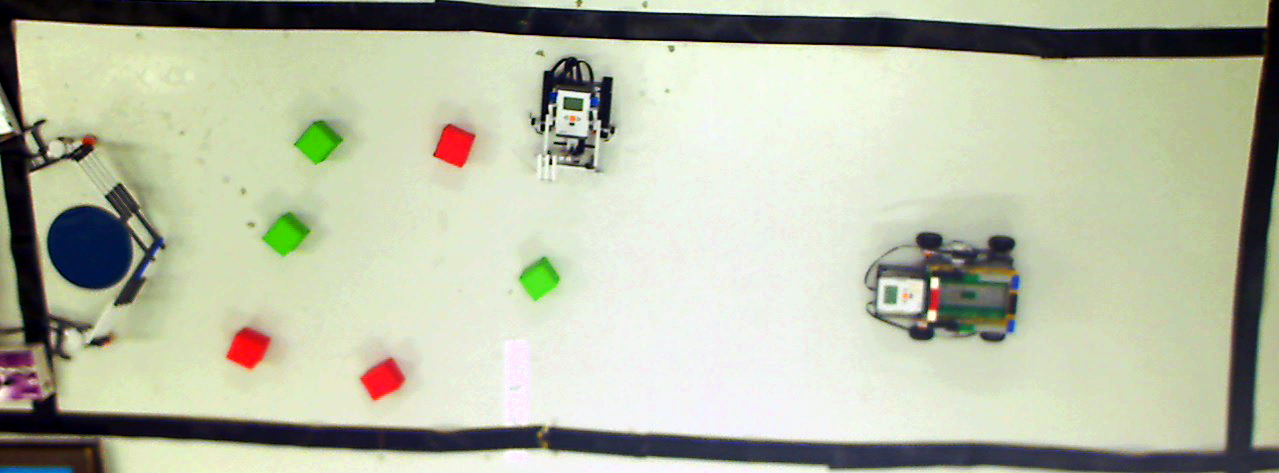
\includegraphics[width=\textwidth]{pictures/photo3development.png}
	\caption{\small The interaction between robots and blocks in development.}
	\label{fig:photo3development}
\end{figure*}

A lot of different situations may arise in this interaction between the robots and the environment. We wrote a piece of pseudo-code that shows the logic we were planning to solve all of these situations, which can be seen in \aref{alg:multiagent}.

\begin{algorithm}
define transport as the transport robot; \\
define guard as the guard robot; \\
define $p$ as path from transport to the goal; \\
\eIf {transport close enough to goal }
{
transport do nothing; \\
guard do nothing; \\
}
{
\uIf {$p$ has obstacles on or near it}
{
\eIf {path passes directly through obstacle}
{
define $l$ as point next to path, on the side with the least other obstacle;
}
{
define $l$ as location on path nearest to obstacle;
}
\eIf{guard near $l$}
{
define $d$ as location on opposite side of obstacle; \\
guard move to $d$, force action completion before accept new action; \\
transport do nothing; \\
}
{
define $p'$ as path from guard to obstacle, using blocks, goal and transport as navigation mesh geometry. Ignore blocks in a set radius around the obstacle; \\
guard move to first node on $p'$; \\
transport do nothing; \\
}
}
\uElseIf{$p$ has guard on or near it}
{
define $d$ as location a set distance away from the path; \\
\If {$d$ outside world}
{
redefine $d$ as location on opposite point of path; \\
}
guard move to $d$; \\
\eIf {transport near guard}
{
transport do nothing; \\
}
{
transport move to first node on $p$; \\
}
}
\uElse
{
transport move to first node on $p$; \\
guard do nothing;
}
}
\caption{Pseudo-code for the multi-agent and environment interaction.}
\label{alg:multiagent}
\end{algorithm}

\begin{figure}[h]
	\centering
	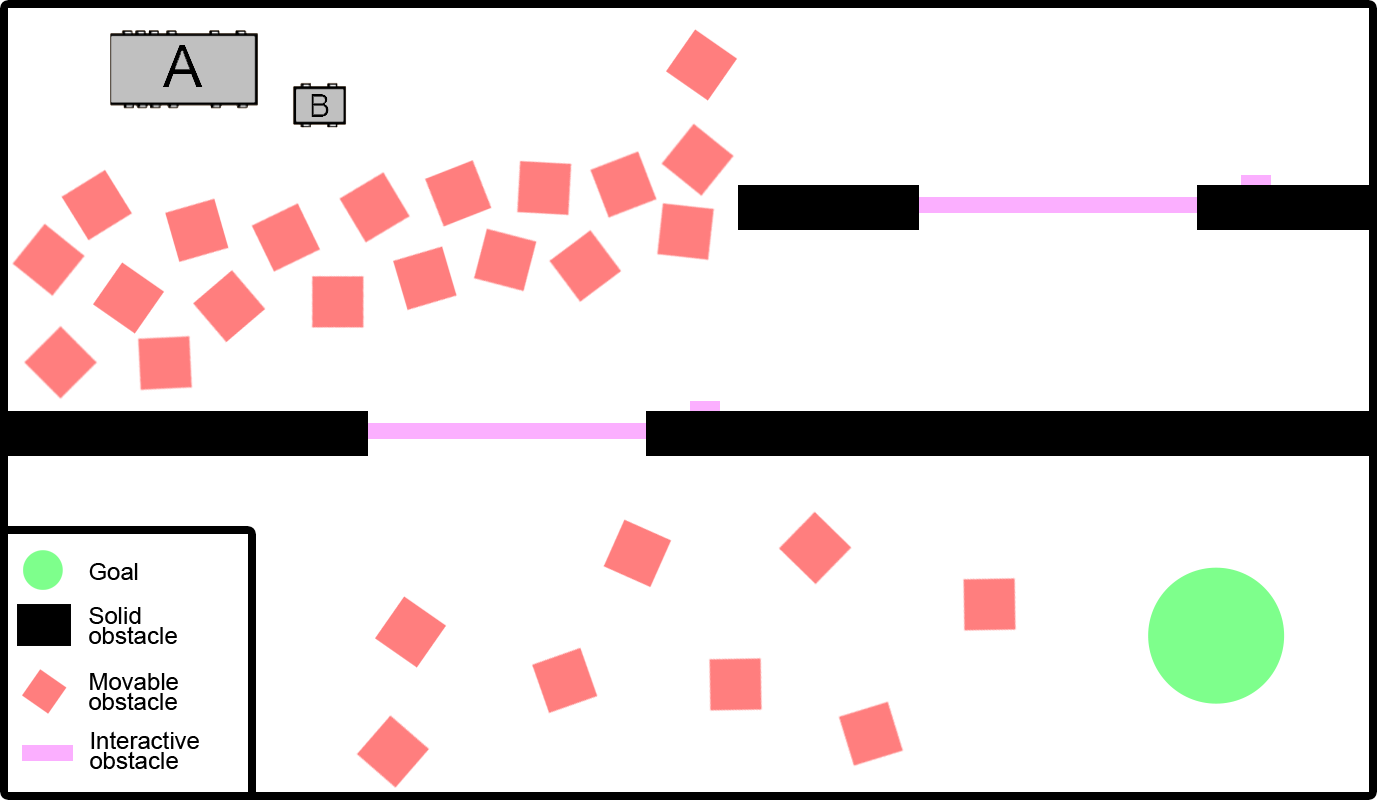
\includegraphics[width=\columnwidth]{pictures/proposalImage.png}
	\caption{\small A mock-up image from our project proposal, containing some ideas that didn't make it into the final project.}
	\label{fig:proposal}
\end{figure}

\subsection{Sockets}
In order to properly separate functionality, our initial plan was to create different applications to handle different things. There would be two robot applications that had capabilities to each issue commands to one of our two robots, and these two applications would receive information from a third application that would handle all image processing and planning. These 3 applications would communicate with each other through sockets.

Sockets are the software-version of the plug and socket used for electricity. One application can send packets to a socket, and another application can receive this packet and answer accordingly. We created several different package types that would determine robot behaviour, such as a "drive forward" packet containing information on the desired speed to drive forward with.

Socket communication did not make it to the final version of our project since it was more of a hassle than a convenience. We ended up doing all of the work in one application, eliminating the risk of bad robot behaviour due to packet loss.

\subsection{Microsoft Robotics Studio}
Microsoft Robotics Studio is a large software package aimed at academic robot control and simulation application development. Choosing to use this package went hand in hand with choosing to use C\# as our language of choice. Robotics Studio proved to be very difficult to set up and use, not to mention the almost impossible task of controlling multiple robots from the same computer.

To ease our pain, we decided to go with another LEGO NXT C\# library (AForge.NET). This turned out to be a great decision since it solved all our Robotics Studio problems in one night.

\subsection{Smart World Model}
Our implementation of a world model contains exactly what you think it would: information on all the objects in the world. This model is updated every time we analyse a camera frame: after all, the position of the goal, robot or walls might have changed. Since we wanted real-time flexibility, we recalculate the entire model every frame. This made for a couple of problems:

\begin{itemize}
\item What if an important object suddenly disappears?
\item How do we cope with insignificant changes? (we want to avoid jitter caused by noisy images)
\item Doesn't this unnecessarily clog up resources?
\end{itemize}

Luckily, the unnecessary use of resources was no problem since this part of the code is insignificant in terms of calculations when compared to the actual analysis of incoming frames. The other two problems however posed significant troubles. Currently, we cope with these through the use of proper image preprocessing and adding certain margins on values that were allowed to be slightly different each time. This method of dealing with these problems is not very robust.

In order to actually achieve robustness in the world model, we thought of something we later dubbed the 'smart world model'. This model would keep track of its previous states, and only update objects when it considered this necessary. This would have cleaned up our code a lot, removing all the random 'magic numbers' and merging everything into one manageable place.

\subsection{Path Refinement}
\label{sec:pathrefinement}
---
MAREIN
---

\subsection{HSV Colour Model}
There are multiple different systems to describe colour. Currently, we're using the common RGB system which defines colours according to their three base components: red, green and blue. We later found that RGB is not ideal to use in real-time image processing because colour fluctuation due to shadows and subtle lighting differences occurs constantly, and this makes for very inconsistent RGB values.

HSV is a different system that describes colours in hue, saturation and value components. HSV is often used in image processing applications because it separates the so-called \textit{luma} (image intensity) information from the \textit{chroma} (colour) information. This makes for a much more robust way to detect colours subject to lighting changes and shadow. Unfortunately, we only found out about this when the majority of our code was already set up to work with RGB data, and it would have taken too much time to rewrite everything.

\subsection{Smaller Robots}
Large robots, while majestic in appearance, come with a downside: they're large. Large robots are impractical to move, generate more momentum which makes them break down more easily (LEGOs are not that tough, unfortunately) and are heavier than smaller specimens. 

We did work around this by replacing our large transport robot with the smaller guard robot, but this was a last minute decision. In the event where we actually would have had two robots, it would have been more practical to have two small robots than a large and a small one.

\subsection{Scale Calibration}
Currently, we calibrate all colours before we start the main process of getting the robot to its goal. The size of objects is different though: every time we tested our project, the webcam was hanging at a different height which in turn made for differing robot sizes. Adding scale calibration would have allowed us to stop using hard-coded estimations for values like the width of the robot, which could have led to more precise pathfinding.

\subsection{Robot Endearment}
We've noticed that people tend to endow the robots we work with during the demonstrations with human emotions such as happiness or anger. Having the robot actually act on these 'emotions' might have been a cool addition; think of happiness when reaching the goal or anger when the goal is moved just before reaching it.

\subsection{EmguCV Data Formats}
\label{sec:emgucvFormats}
As described, we make use of the data formats that EmguCV brings to the table, a necessity when using the library's functionalities. There are two problems with this, with an eye on performance.

First, the EmguCV formats are not optimized for our purposes. For example, when we are using EmguCV images to store blob information, which are really binary bitmaps. The EmguCV format dictates that the image is at least a greyscale image, which is unnecessary for our purpose of storing binary values. Things such as these may contribute negatively to performance.

Second, we make use of Windows Presentation Foundation (WPF), which is not directly compatible with the EmguCV formats. WPF is a system that facilitates the creation of user interfaces for .NET applications. We use it, among other things, to display results at various stages of the analysis process. Since these results are often in EmguCV formats, they need to be converted before being handled by WPF. This takes time and probably has a large negative impact on performance. Note that one optimization we apply is to only convert the relevant data that the user is looking at, at a particular moment.

We had vague plans of taking the EmguCV formats out of our own code and only converting from and to it when interacting with the EmguCV functionality (which is actually only in very few places). This should provide a boost in performance, and create cleaner code, with only our own representations directly visible, and none of EmguCV's.

\section{Demo Evaluation}
The demonstration we had to carry out during D-Day was pretty successful, despite some potentially major setbacks. The lamp we were using to compensate for shadows broke when we were supposed to demonstrate our project, which made a delay necessary. Through some more tweakage of the webcam software, we managed to pull off a working demonstration anyway.

\section{Team}
\label{sec:team}

\subsection{Workload Distribution}

\begin{samepage}

The task distribution ended up roughly as follows:\\
\nolinebreak
\begin{tabularx}{3.2in}{ l | X }
Caspar & Robot construction, object construction \\ 
Chris & Object construction, bluetooth communication, presentation \\ 
Erik & Sockets, MRDS setup, initial project outline, peer review \\ 
Koen & Image analysis, planning, robot control, bluetooth communication, report \\ 
Marein & Image analysis, planning, robot control, report \\
\end{tabularx}\\

\end{samepage}

A more detailed overview of participation in the project regarding code production can be found on the \link{https://github.com/MareinK/robotica2}{GitHub repository}.

\subsection{Personal Remarks}
This section will provide some personal remarks by every team member, indicating how they feel about the finished project, the team effort and so on.

\subsubsection{Caspar}


\subsubsection{Chris}
I think that most of the problems in this project were created by an unfair division of tasks and bad communication between the group members. In the beginning we divided the tasks, Marein en Koen got the overwhelming task of doing the images processing. I think when we divided these tasks nobody expected that this would become by far the biggest part of the project. And although people did not mind helping, helping was hard because Marein and Koen were the ones best familiar with their code.  

Personally I think that some problems could have been avoided by working more together as a group instead of dividing the taks. This way people would have communicated better and the workload distribution would have been divided fairer.  

\subsubsection{Erik}
My experience of this project was that almost all of our plans fell through in practice. We did make a very conscious choice in the beginning to aim for ambition in some areas, but not in others. We chose to put a lot of our complexity into the software part (image processing), and make ourselves as independent of the robot hardware as possible. In retrospect, that probably saved the project. The most unpredictable part of robotics is usually: migrating a concept from the test environment into the real world. Through our approach, the real world could be kept out of the equation for the most part.

I think the biggest problem we really had was project management and communication. For varying reasons, no-one stepped up to lead the project or to coordinate our efforts. This led to poor communication, which led to an uneven distribution of the work-load and tensions, despite the fact that every member had a sincere desire to make the project a success. I’ve given this quite a bit of thought, but am not yet sure how I would solve this in the future. 

\subsubsection{Koen}
It took me quite a long time to realize that our initial project proposal was way too ambitious. This, combined with our late start, sealed the deal: the initial idea was not going to be finished. We still tried to actually incorporate most of the ideas we had until the last moment, but decided to stick to one robot anyway to ensure a working demonstration. 

I'm happy with what we managed to create, given the team's situation. Workload distribution was nowhere near fair; it's clear something went wrong when a 5-man effort is almost entirely executed by two people. I don't want to blame anyone for that however; we all made our mistakes. I learned a lot, both about AI subjects and teamwork. In projects to come, I will try to make sure that my team stays on track through introducing intermediate deadlines in order to avoid the final sprint that we experienced during this project.

\subsubsection{Marein}

\begin{samepage}

\section{Code}
Our complete codebase can be viewed on GitHub at
\nolinebreak
\begin{center}
\link{https://github.com/MareinK/robotica2}{https://github.com/MareinK/robotica2}
\end{center}

\end{samepage}

The repository contains several projects that were used for testing and prototyping. The latest version of the main program code can be found \link{https://github.com/MareinK/robotica2/tree/master/Code/v1/Main}{here}.

After demo day, we made several small changes to the code that mainly concern comments and source citing. The version of the code that was ran on the actual day can be viewed \link{https://github.com/MareinK/robotica2/tree/f4c68dcab28f35ed3ac389d2fb01d46ae9705ea7/Code/v1/Main}{here}.

Git keeps a complete version history that may give interesting insights into how the project developed. Since we started writing this report (which is also stored in the repository), the commit history has been getting a bit messy. Therefore we suggest looking at the history up to January 16th (demo day), found \link{https://github.com/MareinK/robotica2/commits/master?page=3}{here}.

\section{Miscellaneous Material}

\begin{description}
	\item[\link{http://prezi.com/hay_qlcqdzkp/convoi}{Presentation slides}]
	\item[\link{http://www.youtube.com/watch?v=ngBgZgFv_FU}{Presentation and demonstration video}] Note, explanation is not completely correct
	\item[\link{https://github.com/MareinK/robotica2/issues?state=open}{Issue tracker}] Saw limited use
\end{description}

\end{appendices}

\end{document}
